
\newpage
\slidetitle{5. Ergebnisse - L-Systeme}
\subsection{Ergebnisse (2)}





\newpage
\begin{center}
	\vfill
	\begin{minipage}[c]{0.45\textwidth}
		\centering
		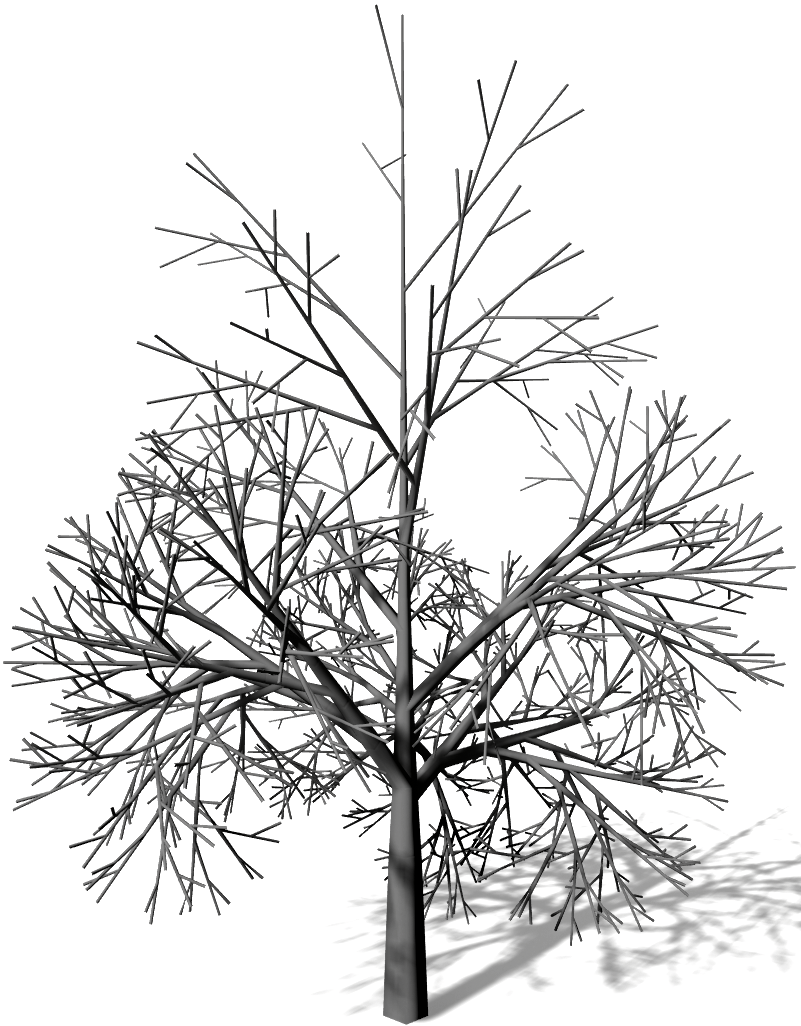
\includegraphics[height=.9\textheight]{images/LS_Monopodial_1}
	\end{minipage}
	\hspace{.05\textwidth}	
	\begin{minipage}[c]{0.45\textwidth}
		\centering
		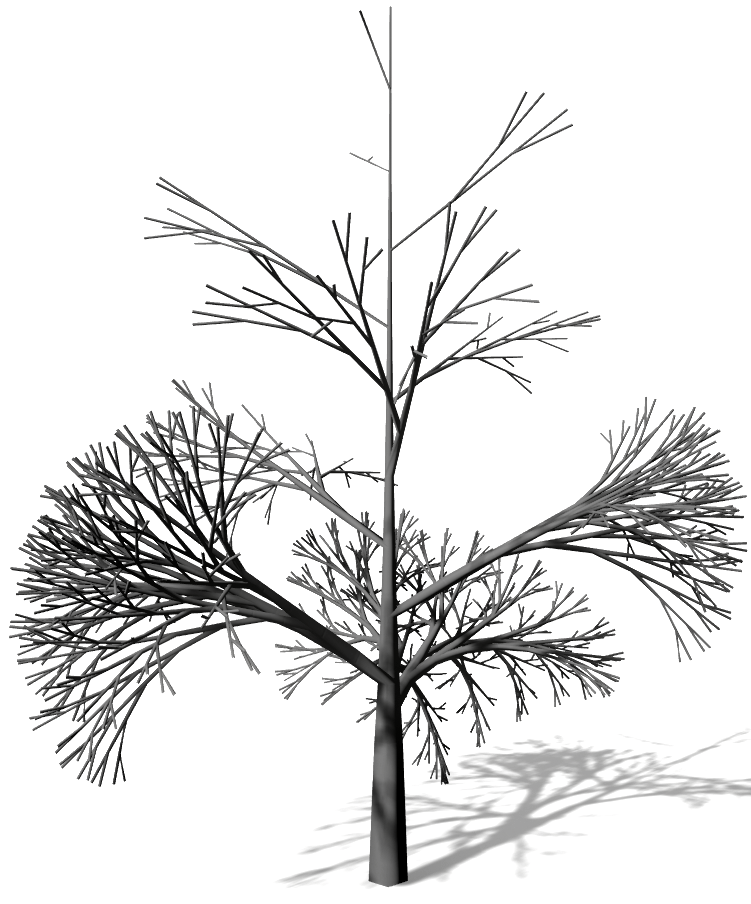
\includegraphics[height=.9\textheight]{images/LS_Monopodial_2}
	\end{minipage}
	\vspace{0.05\textheight}
	
	Monopodiales Wachstum
\end{center}







\newpage
\begin{center}
	\vfill
	\begin{minipage}[c]{0.45\textwidth}
		\centering
		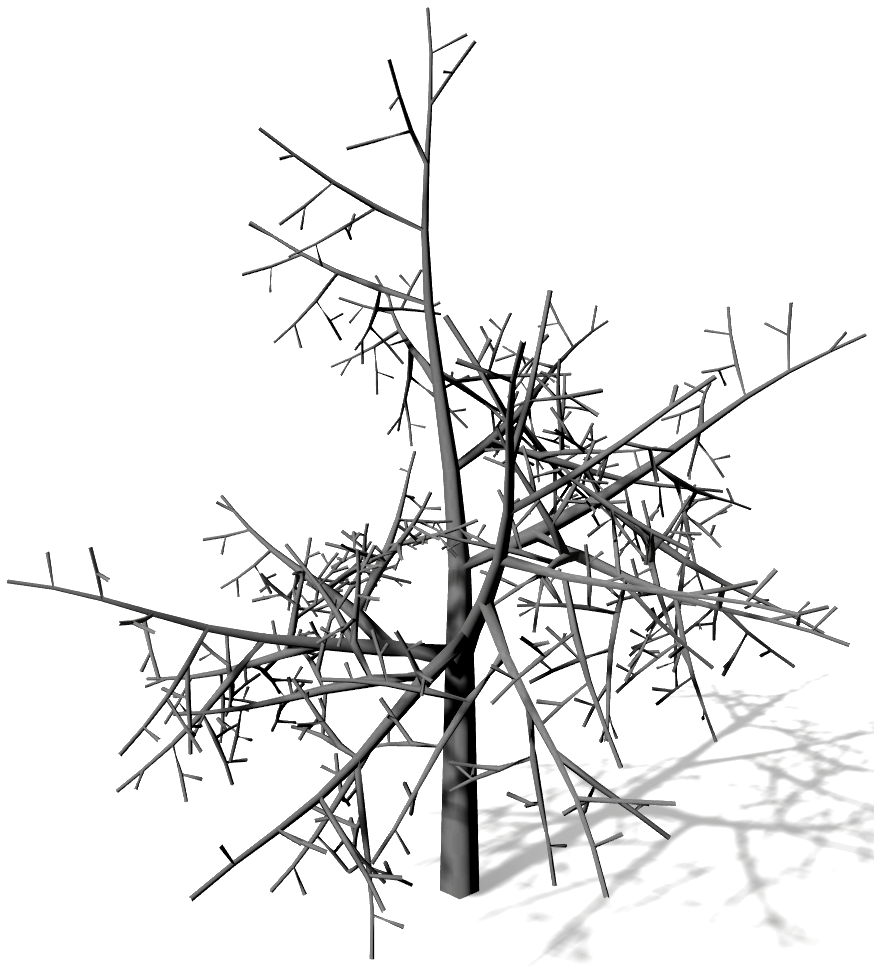
\includegraphics[height=.9\textheight]{images/LS_Sympodial_1}
	\end{minipage}
	\hspace{.05\textwidth}	
	\begin{minipage}[c]{0.45\textwidth}
		\centering
		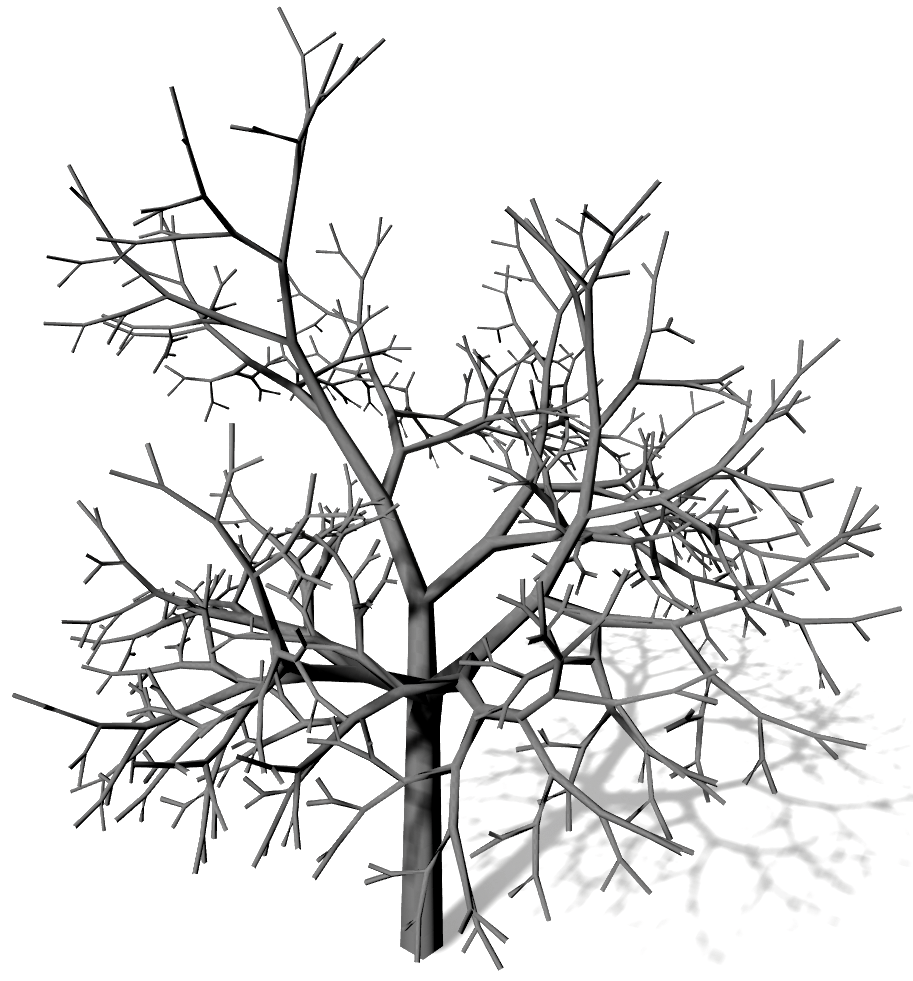
\includegraphics[height=.9\textheight]{images/LS_Sympodial_2}
	\end{minipage}
	\vspace{0.05\textheight}
	
	Sympodiales Wachstum
\end{center}







\newpage
\begin{center}
	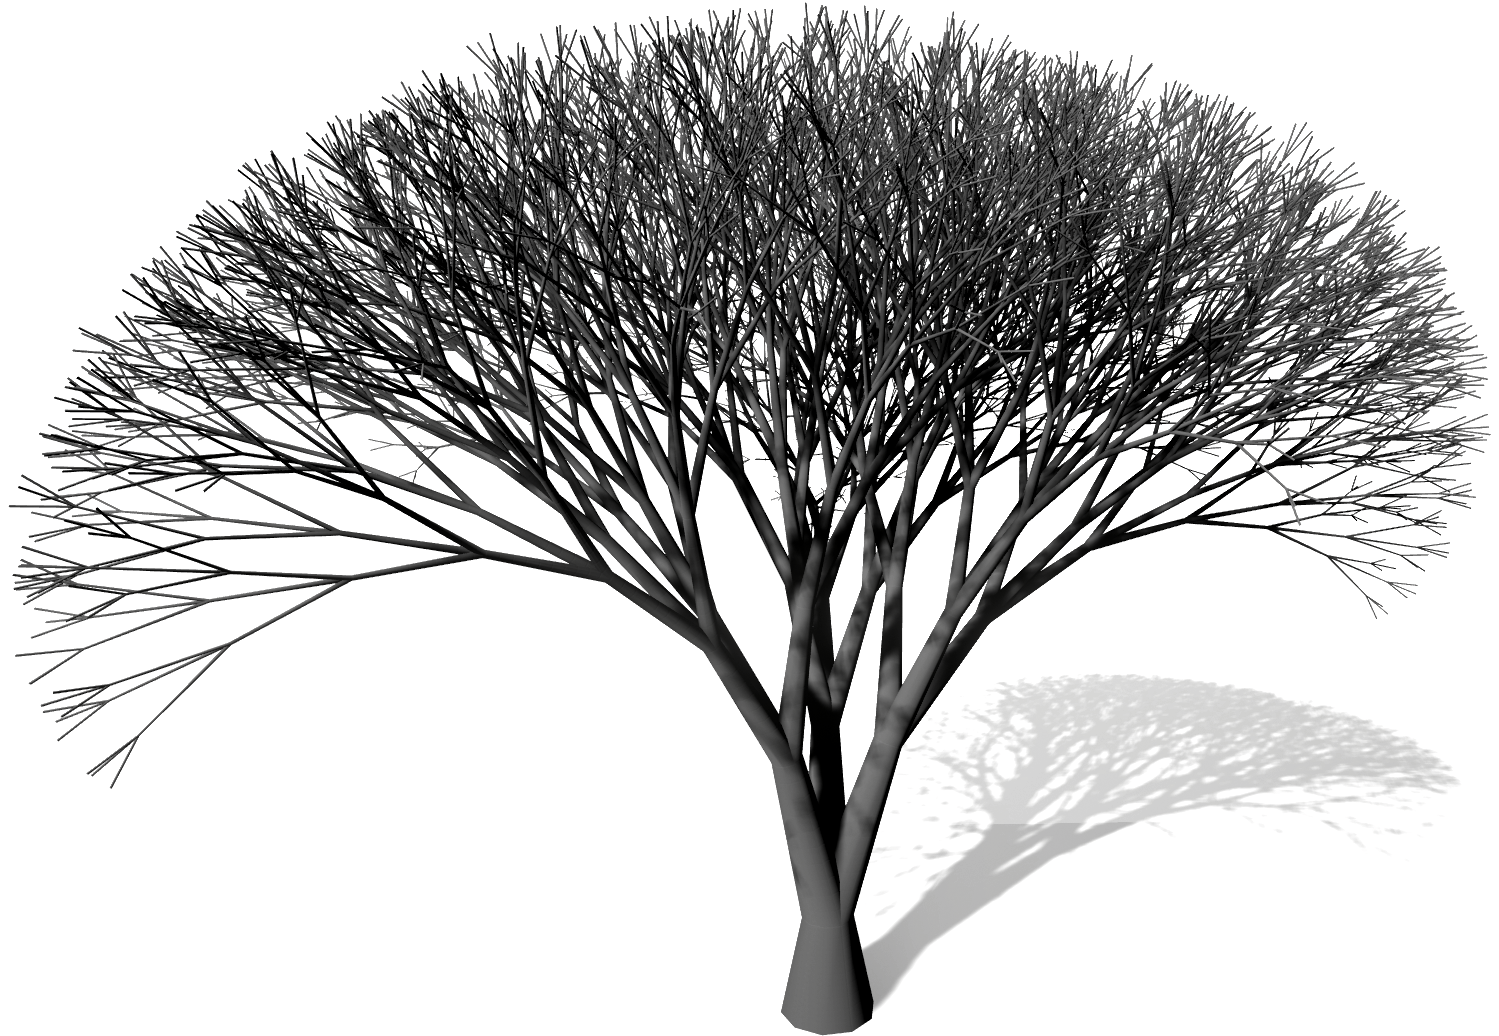
\includegraphics[height=.9\textheight]{images/LS_Ternary_2}
	
	Ternäre Verzweigungen ohne Tropismus
\end{center}






\newpage
\begin{center}
	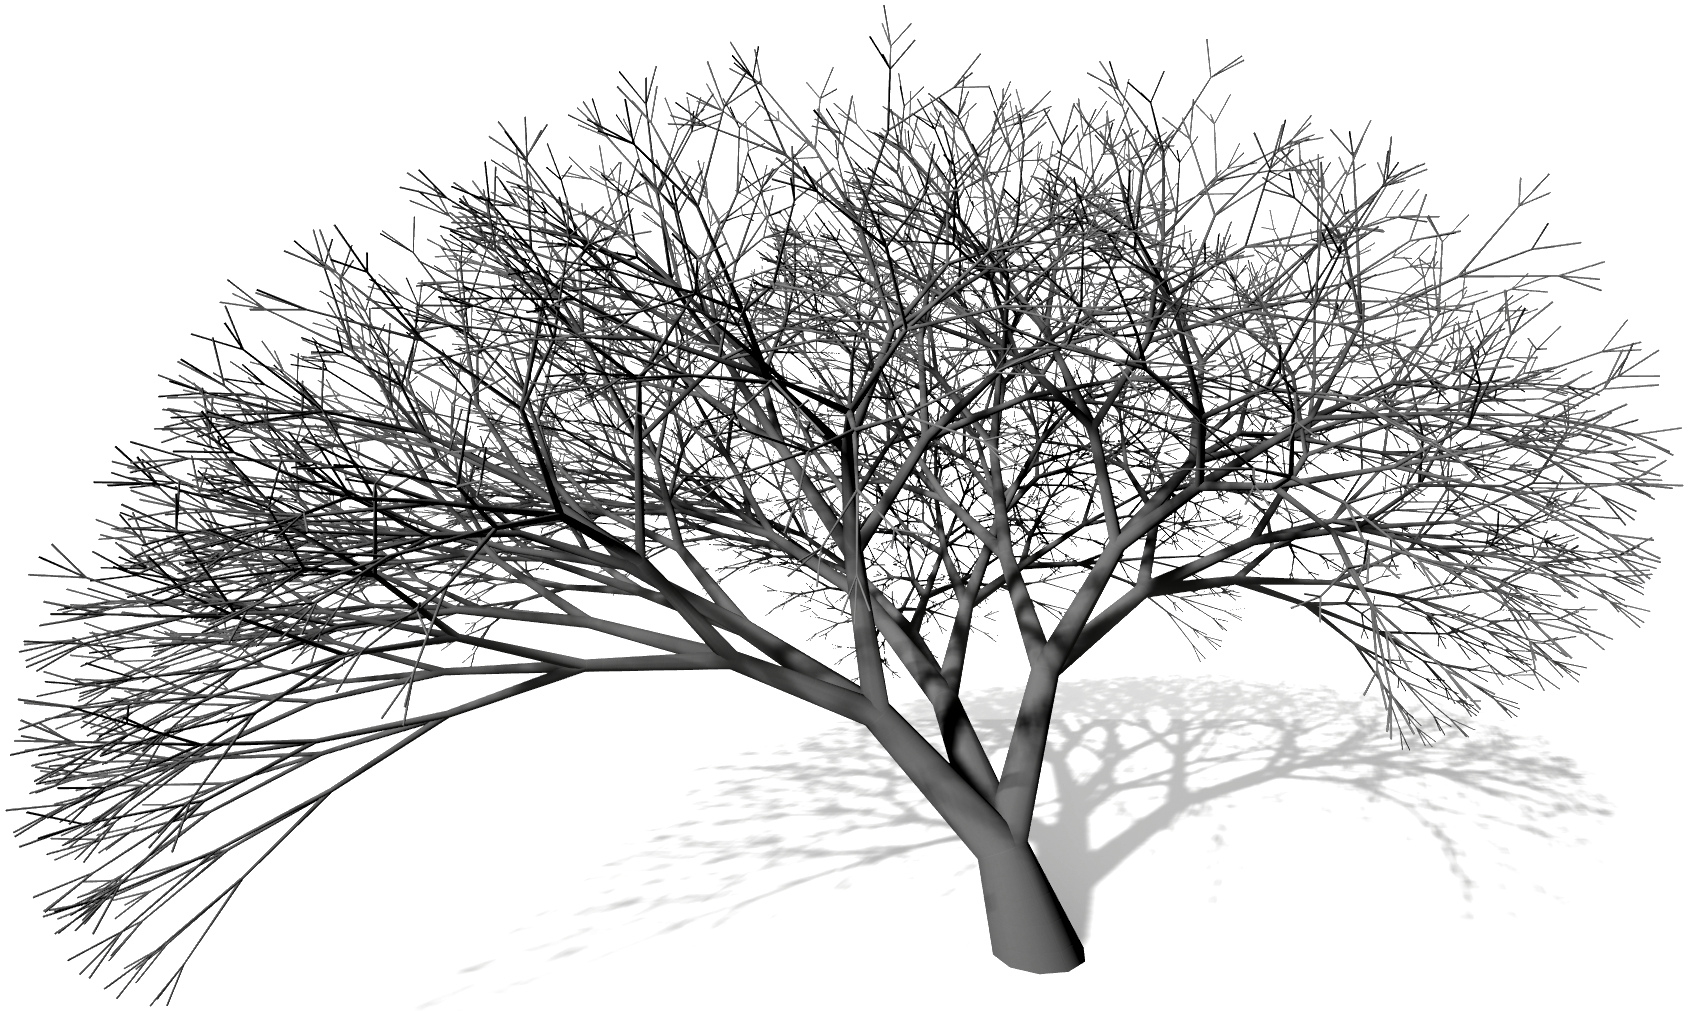
\includegraphics[height=.9\textheight]{images/LS_Ternary_2_Tropism}

	Ternäre Verzweigungen mit Tropismus: $\overrightarrow{T} = (0, -0.5, -1)^T$, $e = 0.5$	
\end{center}








\newpage
\slidetitle{5. Ergebnisse - Space Colonization Algorithmus}
\begin{center}
	\vfill
	\begin{minipage}[c]{0.45\textwidth}
		\centering
		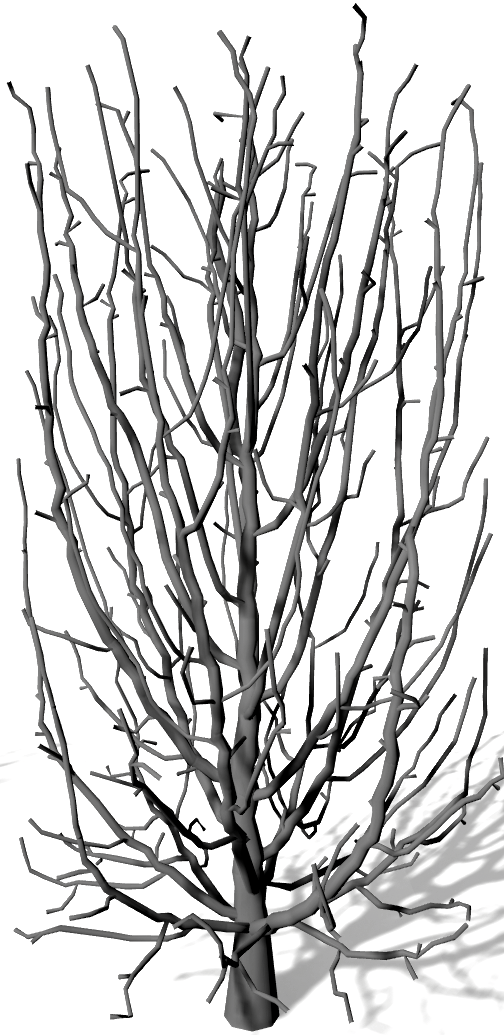
\includegraphics[height=.9\textheight]{images/SCA_Einfluss_Cylinder_High}
	\end{minipage}
	\hspace{.05\textwidth}	
	\begin{minipage}[c]{0.45\textwidth}
		\centering
		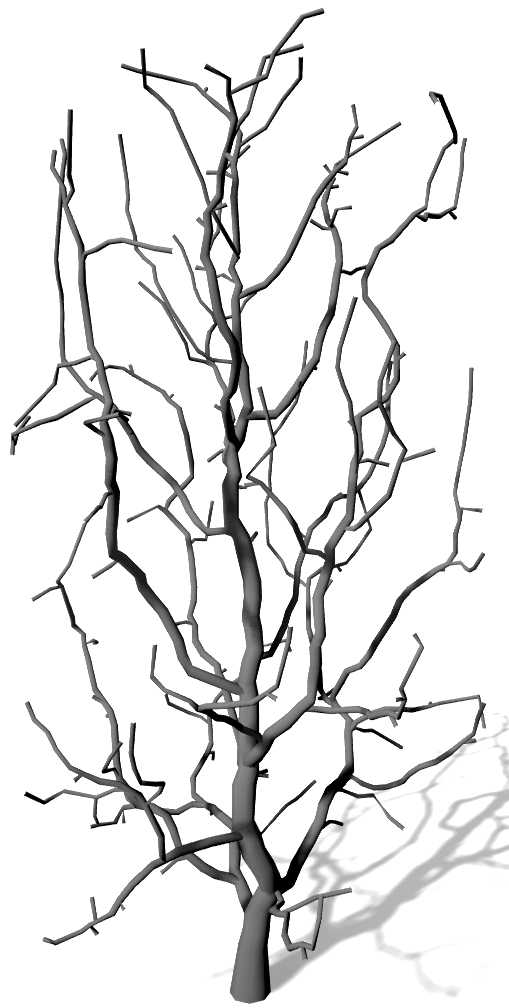
\includegraphics[height=.9\textheight]{images/SCA_Einfluss_Cylinder_Low}
	\end{minipage}
	\vspace{0.05\textheight}

	Form des Einflussbereiches und Anzahl der Einflusspunkte
\end{center}






\newpage
\begin{center}
	\vfill
	\begin{minipage}[c]{0.45\textwidth}
		\centering
		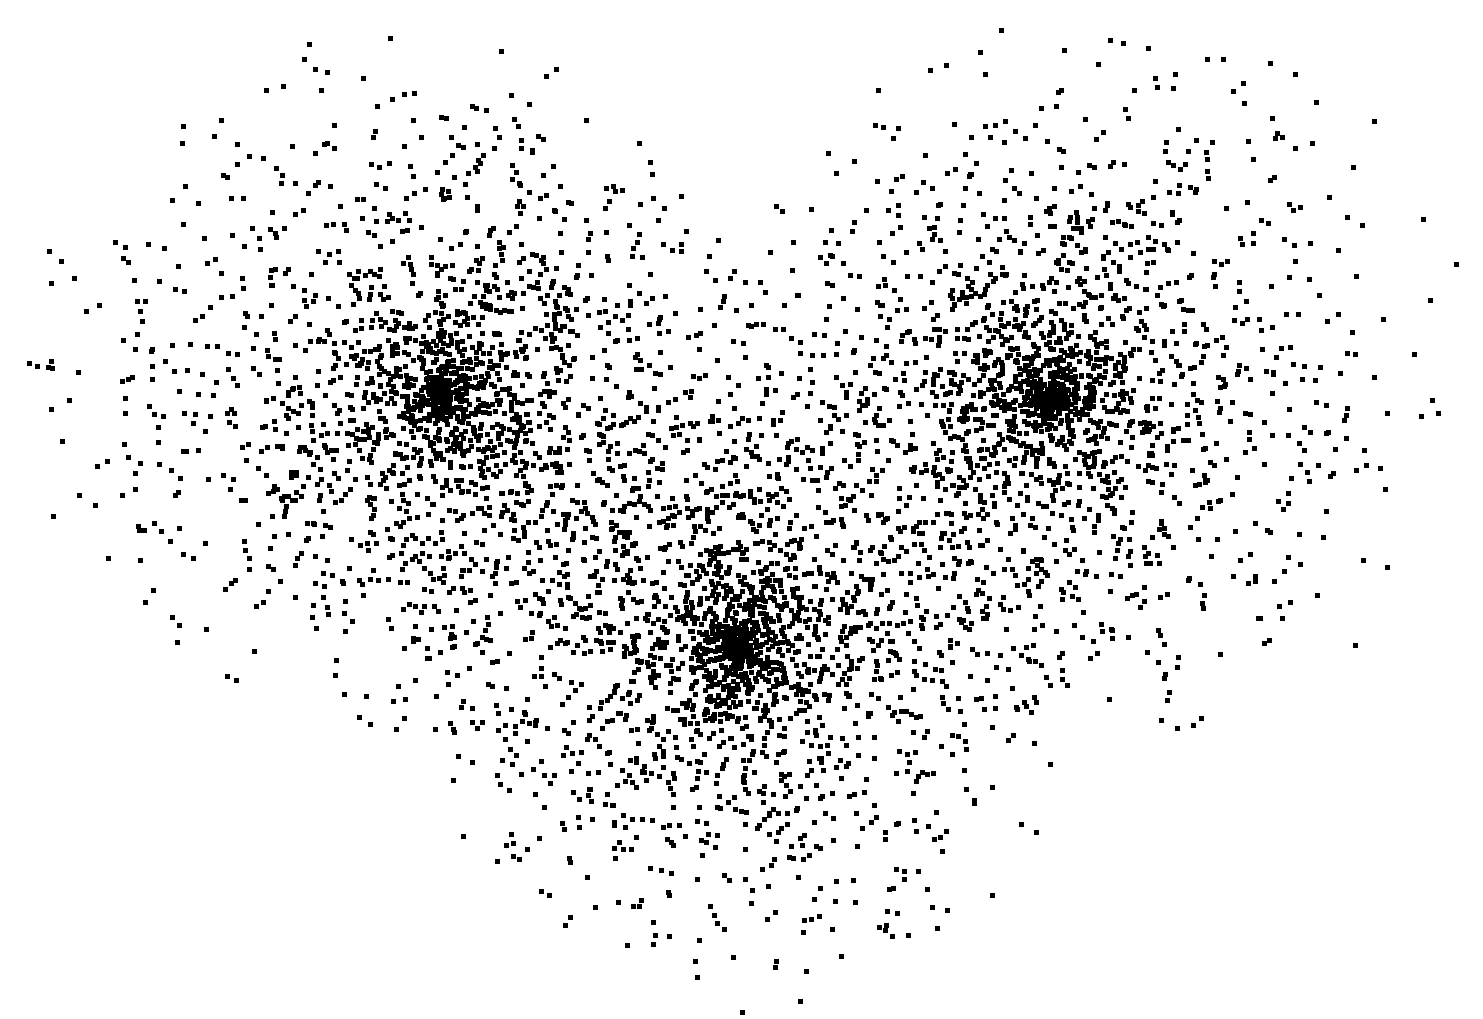
\includegraphics[height=.65\textheight]{images/SCA_MultipleSpheres_Points}
	\end{minipage}
	\hspace{.05\textwidth}	
	\begin{minipage}[c]{0.45\textwidth}
		\centering
		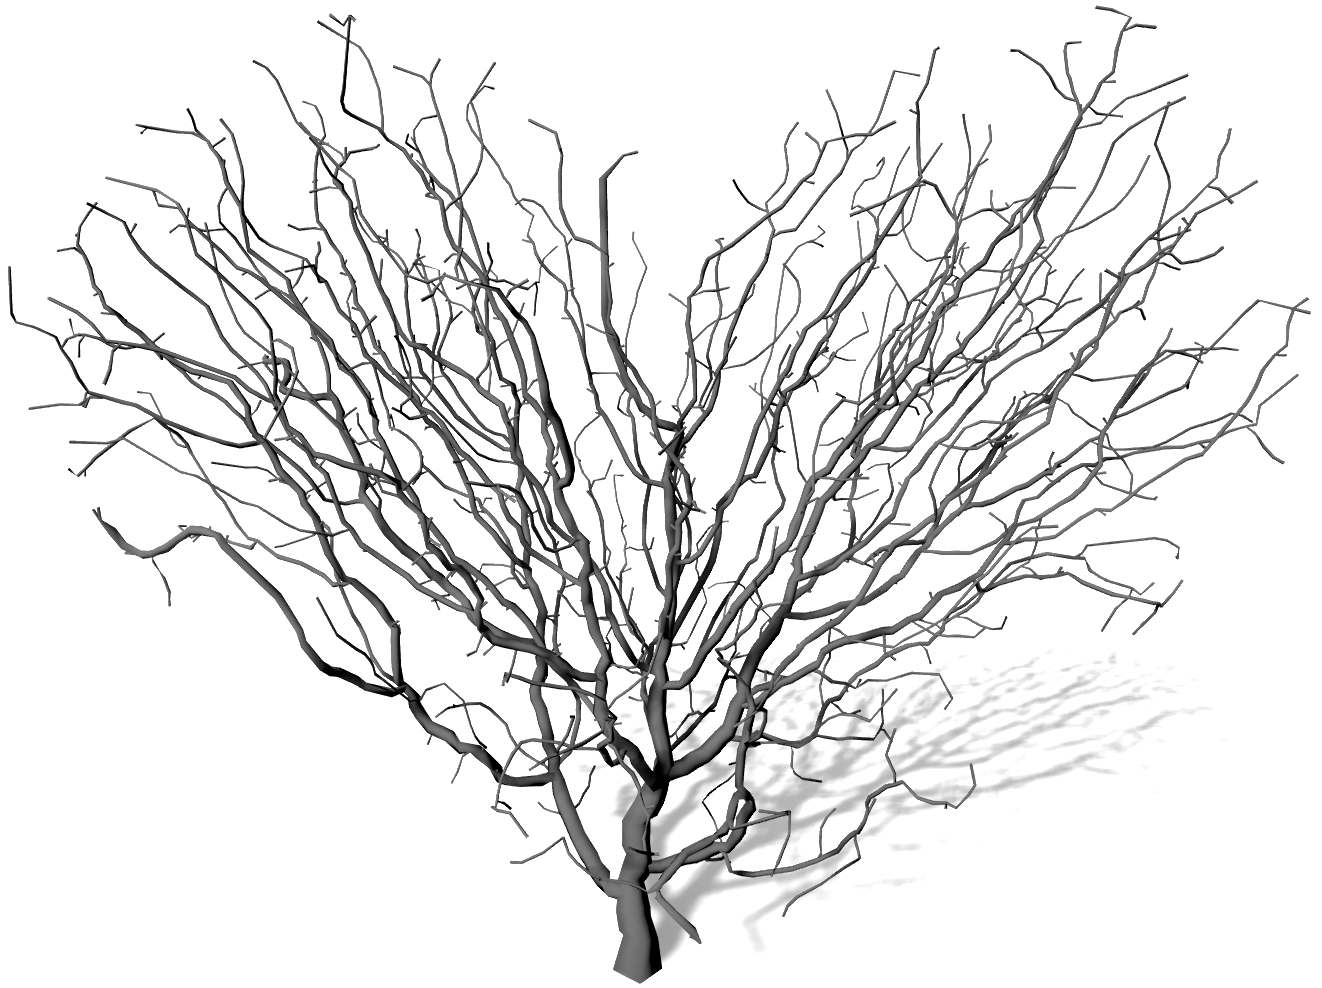
\includegraphics[height=.65\textheight]{images/SCA_MultipleSpheres_Grown}
	\end{minipage}
	\vspace{0.1\textheight}

	Zusammenführen mehrerer Einflussbereiche
\end{center}



\newpage
\begin{center}
	\vfill
	\begin{minipage}[c]{0.45\textwidth}
		\centering
		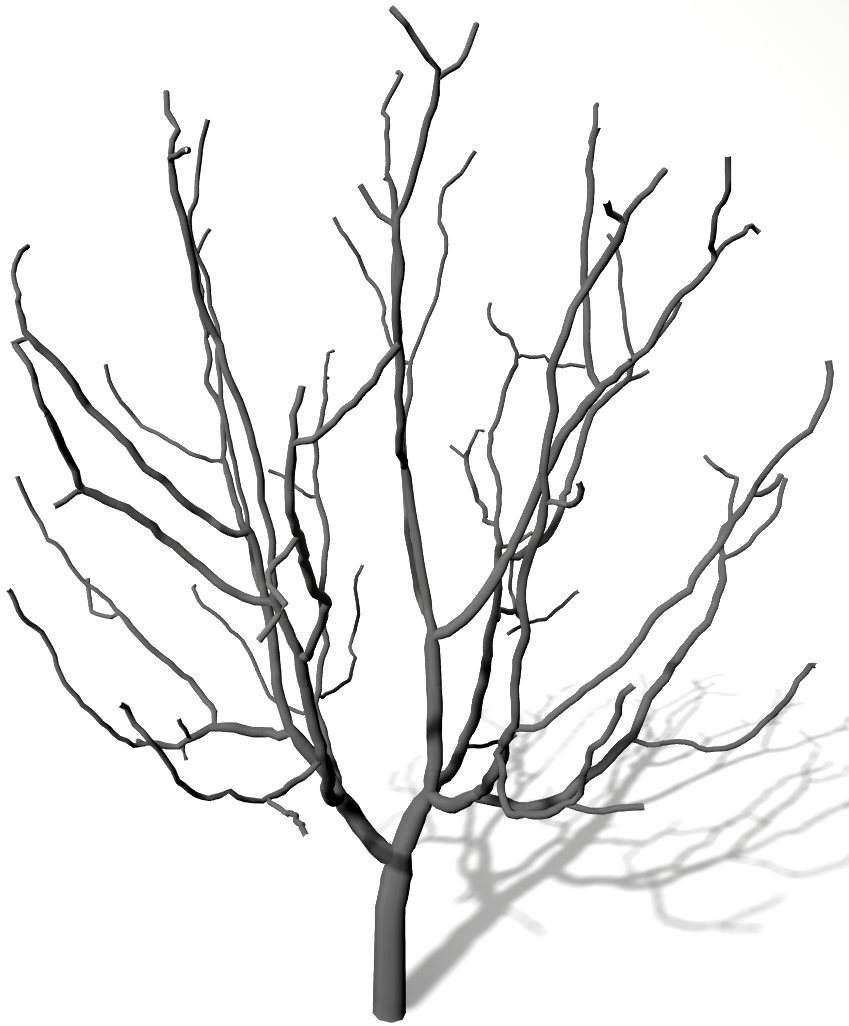
\includegraphics[height=.9\textheight]{images/SCA_KDRI_HighKD_LowRI}
	\end{minipage}
	\hspace{.05\textwidth}	
	\begin{minipage}[c]{0.45\textwidth}
		\centering
		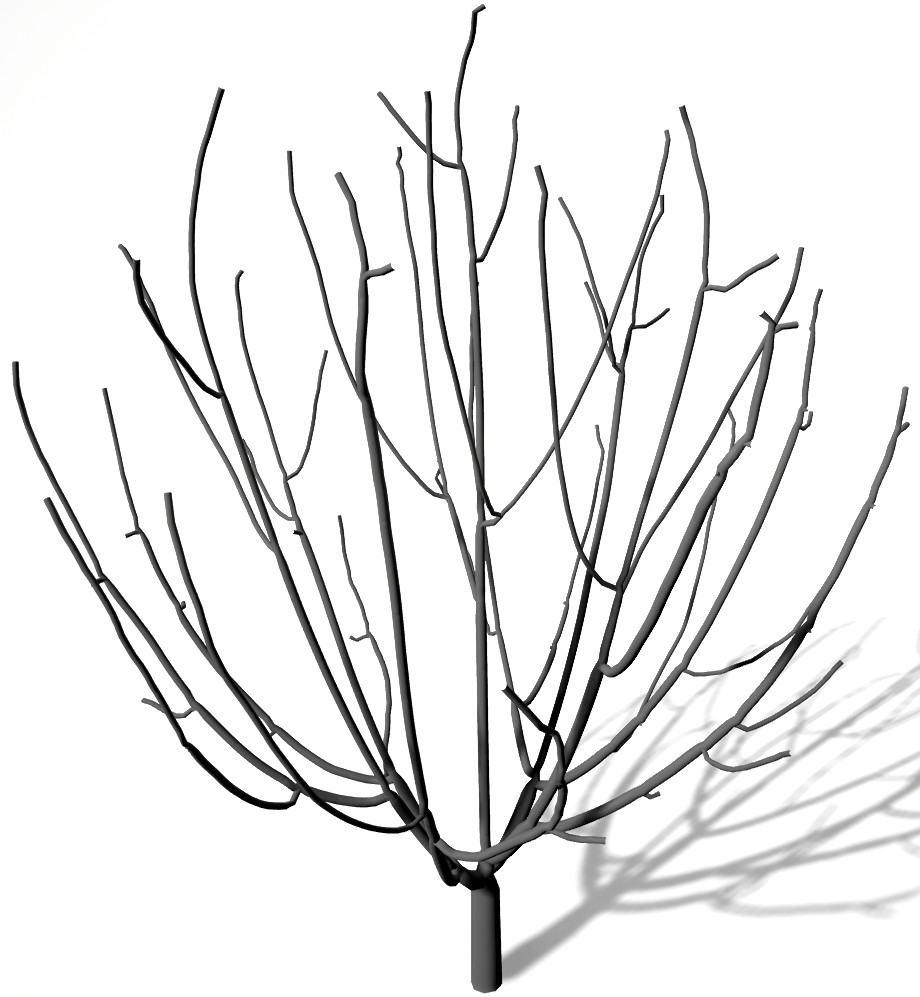
\includegraphics[height=.9\textheight]{images/SCA_KDRI_HighKD_HighRI}
	\end{minipage}
	\vspace{0.05\textheight}
	
	Unterschiedliche Einflussradien
\end{center}





\newpage
\begin{center}
	\vfill
	\begin{minipage}[c]{0.45\textwidth}
		\centering
		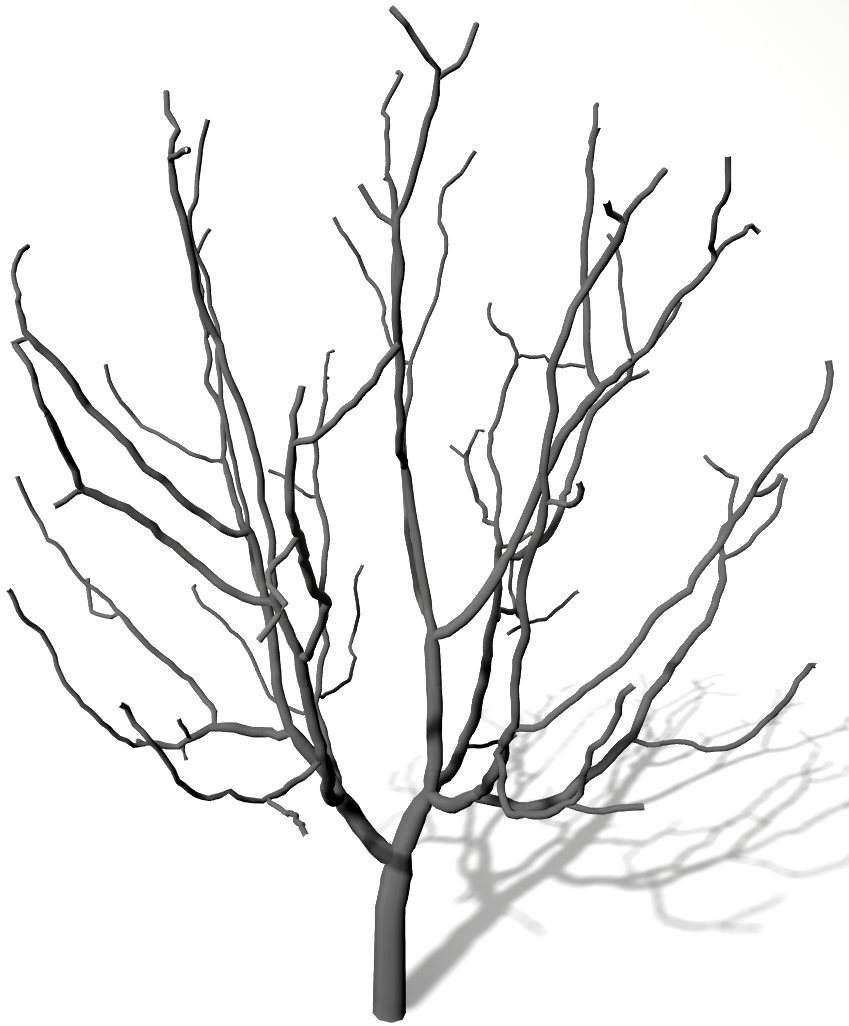
\includegraphics[height=.9\textheight]{images/SCA_KDRI_HighKD_LowRI}
	\end{minipage}
	\hspace{.05\textwidth}	
	\begin{minipage}[c]{0.45\textwidth}
		\centering
		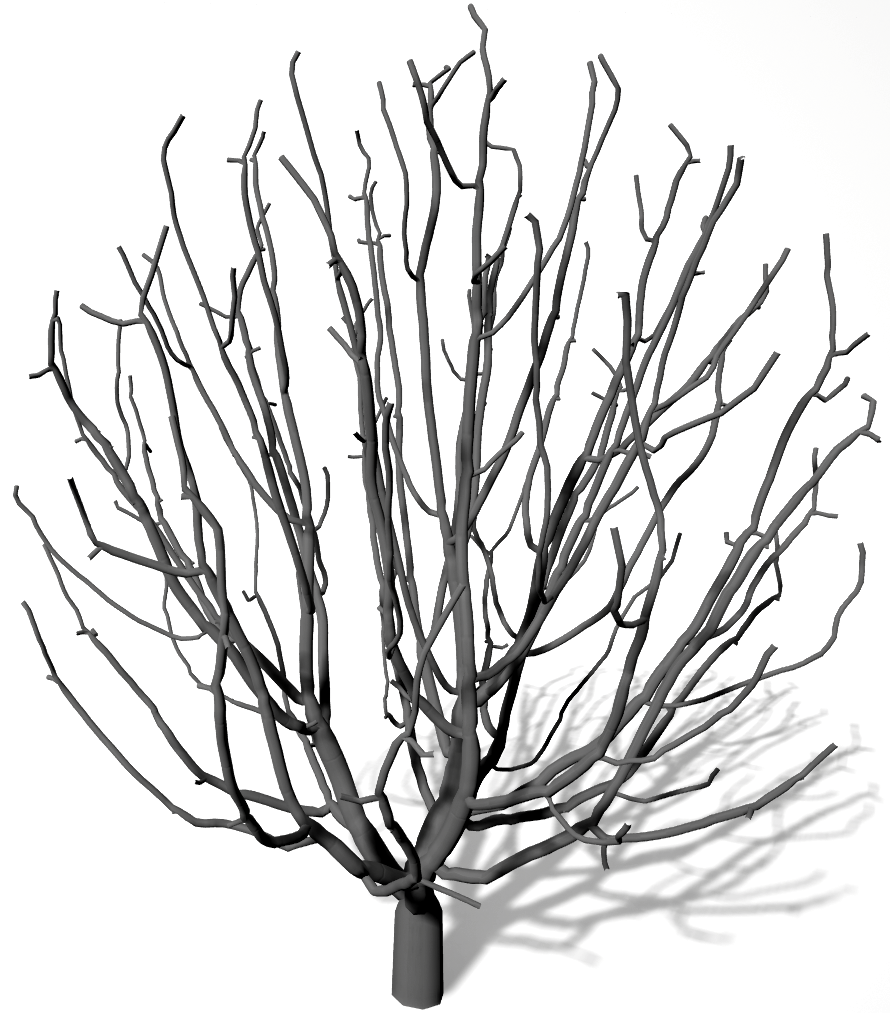
\includegraphics[height=.9\textheight]{images/SCA_KDRI_LowKD_LowRI}
	\end{minipage}
	\vspace{0.05\textheight}
	
	Einfluss des Minimalradius
\end{center}




\newpage
\begin{center}
	\vfill
	\begin{minipage}[c]{0.45\textwidth}
		\centering
		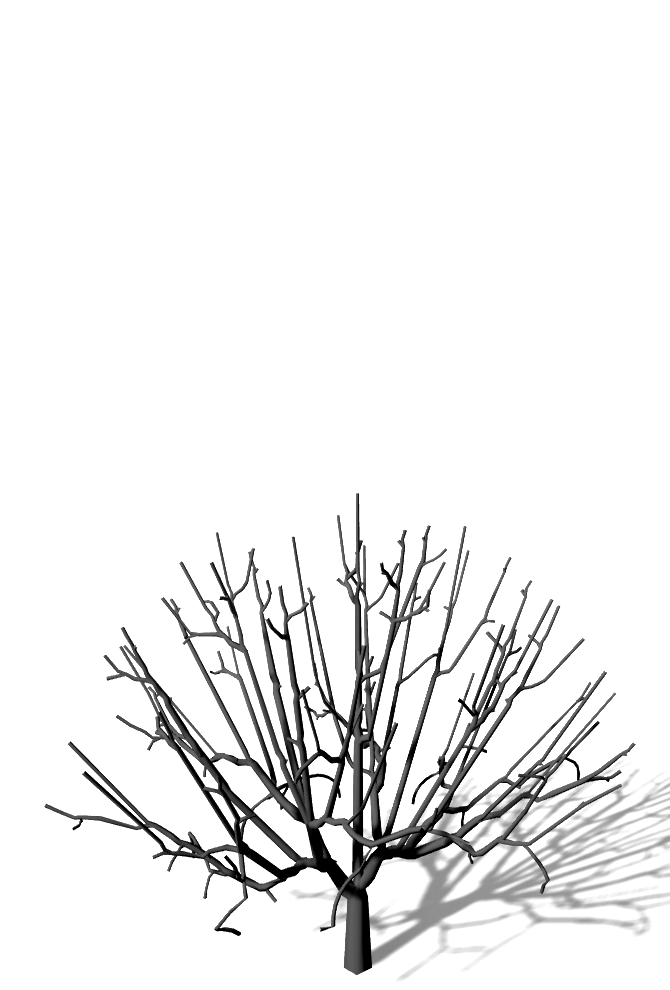
\includegraphics[height=.9\textheight]{images/SCA_GewWachstum_Off}
	\end{minipage}
	\hspace{.05\textwidth}	
	\begin{minipage}[c]{0.45\textwidth}
		\centering
		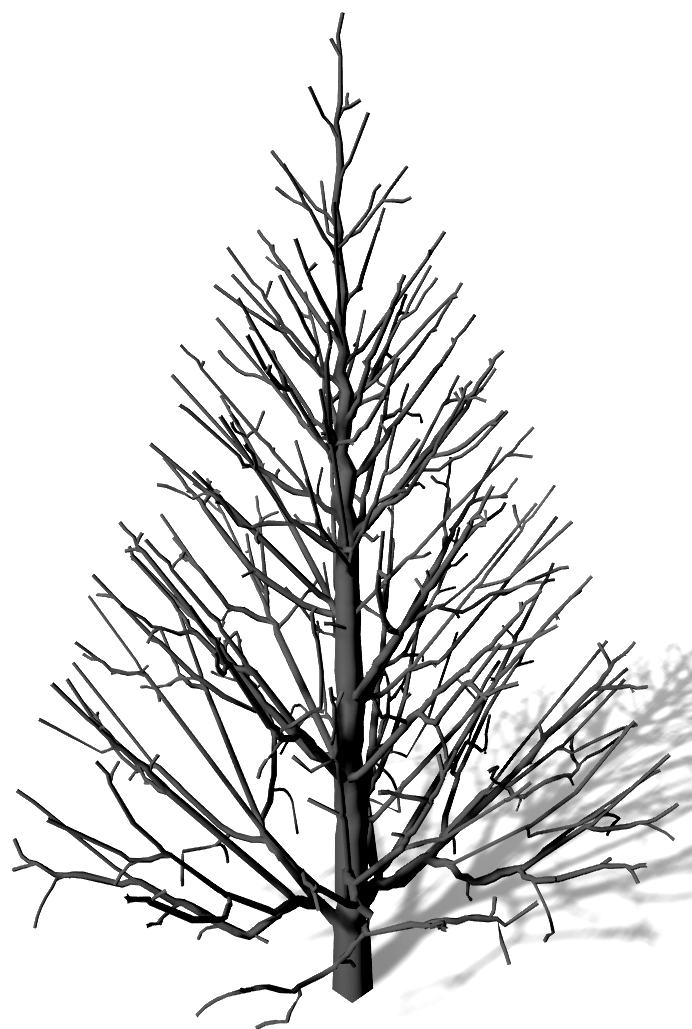
\includegraphics[height=.9\textheight]{images/SCA_GewWachstum_On}
	\end{minipage}
	\vspace{0.05\textheight}
	
	Optimale Verwendung des gewichteten Wachstums
\end{center}
